\documentclass[sigconf,anonymous,review]{acmart}

\setcopyright{none}
\settopmatter{printacmref=false}
\settopmatter{printfolios=true}
\acmConference[KDD 2027]{Proceedings of the 33rd ACM SIGKDD Conference on Knowledge Discovery and Data Mining}{August 1--5, 2027}{San Jose, CA, USA}
\acmISBN{}
\acmDOI{}

\usepackage{booktabs}
\usepackage{graphicx}
\usepackage{amsmath}
\usepackage{multirow}
\usepackage{placeins}
\usepackage{algorithm}
\usepackage{algpseudocode}

\begin{document}

\title{IGV: Incremental Graph Versioning for Efficient\\Retrieval-Augmented Generation over Evolving Corpora}

\author{Anonymous Author(s)}
\affiliation{\institution{Anonymous Institution}
\city{Anonymous City}
\country{Anonymous Country}}

\begin{abstract}
Graph-based Retrieval-Augmented Generation (GraphRAG) enhances large language models (LLMs) by structuring document corpora as knowledge graphs, enabling multi-hop reasoning and global question answering. However, existing GraphRAG systems require expensive full-graph rebuilds when new documents arrive, making them impractical for dynamic, evolving corpora. We present IGV (Incremental Graph Versioner), a framework that supports efficient incremental updates to GraphRAG indexes through three components: (1) embedding-based semantic entity deduplication, (2) embedding-based graph relinking, and (3) incremental community repartitioning with community summary generation for global QA retrieval. Experiments on five multi-hop QA datasets with LLM-based entity extraction (Qwen2.5-7B-Instruct) across 2,000 passages and 120 evaluation questions per dataset demonstrate that IGV achieves 10$\times$ faster updates than full rebuild while maintaining factoid QA quality. Critically, IGV's community summary retrieval improves global QA F1 by 12.6--93.8\% over naive incremental baselines on 3/5 datasets, and even surpasses VectorRAG on streaming corpora. All methods share cached LLM entity extractions, ensuring fair ablation comparisons.
\end{abstract}

\keywords{GraphRAG, Incremental Indexing, Knowledge Graph, Retrieval-Augmented Generation}

\maketitle

\section{Introduction}

Retrieval-Augmented Generation (RAG) mitigates LLM hallucinations by grounding responses in retrieved external knowledge. While traditional vector RAG excels at factoid lookups, it struggles with global questions requiring cross-document reasoning---questions such as ``What are the main themes across this document collection?'' or ``How are these entities related?'' GraphRAG addresses this limitation by constructing knowledge graphs from text corpora, enabling structured multi-hop retrieval and community-level summarization~\cite{edge2024graphrag,guo2025lightrag}. By organizing entities and their relationships into a graph index, GraphRAG systems can answer queries that require synthesizing information across multiple documents, which flat vector retrieval cannot handle effectively.

The core workflow of GraphRAG consists of three phases: (1) \emph{offline indexing}, where an LLM extracts entities and relationships from each document, building a knowledge graph; (2) \emph{community detection}, where the graph is partitioned into thematic communities, each summarized by the LLM; and (3) \emph{online retrieval}, where queries are answered by matching entities (for specific questions) or community summaries (for global questions). This architecture enables both factoid QA (via entity-level retrieval) and global QA (via community-level summarization), a capability that vector RAG fundamentally lacks.

A critical limitation of current GraphRAG systems is their reliance on \emph{full rebuilds} for corpus updates. Microsoft GraphRAG~\cite{edge2024graphrag} requires re-running entity extraction, community detection, and summary generation over the entire corpus when any new document arrives. For a 5,000-passage corpus, this costs over 4.5 hours of LLM time and significant API expenditure. LightRAG~\cite{guo2025lightrag} introduced a set-union incremental update mechanism that avoids full rebuilds, but its naive merging approach creates three problems: (1) duplicate entities---the same real-world entity extracted from different documents with slightly different surface forms creates redundant nodes; (2) disconnected graph components---new entities are added without connecting them to the existing graph structure; and (3) stale communities---community assignments computed on the initial corpus become outdated as new entities arrive, degrading global query performance.

These problems compound over time: with each incremental batch, the graph becomes increasingly bloated with duplicates, fragmented across disconnected components, and organized into communities that no longer reflect the current graph structure. This degradation directly impacts retrieval quality, and the cost of full rebuild makes GraphRAG impractical for streaming applications such as news monitoring, enterprise knowledge base maintenance, and scientific literature tracking.

We propose IGV (Incremental Graph Versioner), which addresses these problems through three components: semantic entity deduplication using sentence-transformer embeddings, embedding-based graph relinking that connects semantically similar entities, and incremental community repartitioning with LLM-generated community summaries for global QA retrieval. The key insight is that community summaries provide a thematic index for global questions, which factoid retrieval cannot serve effectively. Unlike prior work that treats community detection as an offline preprocessing step, IGV maintains communities incrementally and leverages them at query time through community summary retrieval.

Our contributions are as follows:
\begin{itemize}
\item We formulate the incremental GraphRAG maintenance problem and identify three challenges: entity duplication, graph fragmentation, and community staleness.
\item We propose IGV, combining embedding-based deduplication, semantic relinking, and incremental community repartitioning with community summary generation.
\item We introduce a fair ablation methodology using cached LLM entity extractions, eliminating the non-determinism that invalidated prior comparisons.
\item We evaluate on five datasets with two QA modes (factoid and global), demonstrating 10$\times$ efficiency and 12.6--93.8\% global QA improvement on 3/5 datasets.
\end{itemize}

\section{Related Work}

\textbf{GraphRAG Systems.} Edge et al.~\cite{edge2024graphrag} proposed GraphRAG, which builds entity knowledge graphs via LLM extraction, applies Leiden community detection~\cite{traag2019leiden}, and generates community summaries for global query answering. Their system processes documents in two phases: offline indexing and online query. While effective for static corpora, the system requires complete re-indexing when new documents arrive, with cost proportional to the entire corpus size. LightRAG~\cite{guo2025lightrag} simplified this with a dual-level retrieval paradigm and introduced basic incremental updates via set union, but lacks deduplication, relinking, and incremental community maintenance. Their dual-level retrieval (entity-level and relation-level) inspired our factoid retrieval design. PathRAG~\cite{chen2026pathrag} introduced flow-based path pruning to reduce retrieval redundancy, complementing our community-based approach. HippoRAG~\cite{gutierrez2024hipporag} used Personalized PageRank for neurobiologically inspired retrieval, offering an alternative graph traversal strategy that we include as a baseline (HippoRAG). GNN-RAG~\cite{mavromatis2025gnnrag} combined graph neural networks with LLMs for KGQA, learning node representations for retrieval. GRAG~\cite{hu2025grag} addressed networked document retrieval by modeling inter-document relationships. ReGraphRAG~\cite{kim2025regraphrag} reorganized fragmented knowledge graphs through entity consolidation, sharing conceptual similarities with our deduplication stage. GFM-RAG~\cite{luo2025gfmrag} proposed a graph foundation model for RAG, pre-training on diverse graph structures. LEGO-GraphRAG~\cite{cao2024lego} modularized the GraphRAG pipeline into independent components, enabling flexible deployment. Comprehensive surveys~\cite{peng2025graphsurvey,han2024graphrag} provide systematic overviews of the GraphRAG landscape. Think-on-Graph~\cite{sun2024tog} and its successor~\cite{ma2025tog2} proposed interactive KG reasoning with LLMs, using the KG as a reasoning scaffold rather than a retrieval index. Simple is Effective~\cite{li2025simple} analyzed the roles of graphs and LLMs in KG-based RAG, finding that graph structure benefits global but not always factoid QA---consistent with our observations. G-Retriever~\cite{he2024gretriever} enabled chatting with textual graphs through subgraph retrieval.

\textbf{RAG Fundamentals and Applications.} Lewis et al.~\cite{lewis2020rag} introduced RAG for knowledge-intensive NLP tasks, establishing the retrieve-then-generate paradigm. KG-guided RAG~\cite{zhu2025kguided} used KG semantics for query disambiguation. Paths-over-Graph~\cite{tan2025paths} extracted reasoning paths from KGs. Domain-specific applications include medical~\cite{wu2024junde,zhao2025medrag,liu2025detecting}, financial~\cite{sarmah2024hybridrag}, customer service~\cite{xu2024kgrag}, recommendation~\cite{wang2025kgragrec}, and multimodal~\cite{bu2025querydriven,lee2024multimodal,liang2024multimodal} settings. KG alignment~\cite{tian2025systematic} and personalization~\cite{prahlad2025personalizing} have also been explored. LLM-based KG construction~\cite{zhang2024extract,hofer2024construction} and hallucination reduction~\cite{agrawal2024hallucination} are active research areas. Graph-of-Thoughts~\cite{besta2024got}, MindMap~\cite{wen2024mindmap}, and graph neural prompting~\cite{tian2024gnn} bridge graph structures with LLM reasoning. Generate-on-Graph~\cite{yao2024gog} treats LLMs as both agent and KG.

\textbf{Incremental and Continual Learning.} GORAG~\cite{wang2025gorag} proposed online graph updates for social media classification, addressing dynamic graph construction but without community-level reasoning. KAG~\cite{liang2024kag} introduced logical-form-guided reasoning with schema constraints. Practical GraphRAG~\cite{min2025practical} reduced construction cost via dependency parsing. Continual graph learning~\cite{yuan2026continual} and dynamic GNNs~\cite{zheng2024dynamic} address evolving graph structures but focus on representation learning rather than retrieval. Continual learning for LLMs~\cite{wu2024continual} surveys knowledge update strategies. Incremental learning approaches include exemplar replay~\cite{zhang2024influential}, sub-graph distillation~\cite{fan2024dynamic}, and high-order experience replay~\cite{wang2024continual}. Temporal KGQA methods~\cite{gao2024twostage,qian2024timer} handle time-aware reasoning. GNN explainability~\cite{longa2024explaining} is studied for model transparency. Community detection algorithms~\cite{blondel2008louvain,traag2019leiden} provide the algorithmic foundation for our incremental repartitioning. Louvain~\cite{blondel2008louvain} optimizes modularity through local node reassignment, while Leiden~\cite{traag2019leiden} guarantees well-connected communities. Both operate on the full graph, making incremental variants essential for dynamic corpora.

\section{Methodology}

\subsection{Problem Formulation}

Given a knowledge graph $G = (V, E)$ constructed from an initial document corpus $\mathcal{D}_0$, and a stream of new document batches $\mathcal{D}_1, \mathcal{D}_2, \ldots, \mathcal{D}_T$ arriving over time, the goal is to update $G$ to incorporate new entities and relationships from each batch $\mathcal{D}_t$ while satisfying four objectives:
\begin{enumerate}
\item \textbf{Efficiency:} Minimizing LLM calls per update, the dominant cost in GraphRAG.
\item \textbf{Consistency:} Avoiding duplicate entities that fragment the graph.
\item \textbf{Community quality:} Maintaining community structure that reflects the current graph topology.
\item \textbf{Retrieval utility:} Preserving factoid QA quality while improving global QA through community-level reasoning.
\end{enumerate}

The full rebuild approach processes all documents $\bigcup_{i=0}^{t} \mathcal{D}_i$ from scratch at each step, with cost $O(\sum_{i=0}^{t} |\mathcal{D}_i|)$ LLM calls. The naive incremental approach (LightRAG) processes only the new batch $\mathcal{D}_t$, with cost $O(|\mathcal{D}_t|)$, but sacrifices graph consistency and community quality. IGV achieves the same $O(|\mathcal{D}_t|)$ LLM cost while maintaining consistency through deduplication, connectivity through relinking, and community quality through incremental repartitioning.

\subsection{IGV Architecture}

IGV processes each incremental batch $\mathcal{D}_t$ through four sequential stages, as formalized in Algorithm~\ref{alg:igv}.

\textbf{Stage 1: LLM-Based Entity Extraction.} For each new document $d \in \mathcal{D}_t$, Qwen2.5-7B-Instruct extracts named entities and their relationships as triplets $(s, r, o)$, where $s$ and $o$ are entity mentions and $r$ is the relationship description. The extraction prompt instructs the LLM to identify people, organizations, locations, concepts, and other named entities, returning results as a JSON list. Each entity is augmented with a description derived from its surrounding context. A document node (DOC\_$d$) is created for each document, connecting all entities extracted from it. A critical design choice is that entity extraction results are \emph{cached} and shared across all methods, ensuring that ablation comparisons reflect only graph construction differences, not LLM non-determinism. This is essential because LLM-based extraction is non-deterministic: without caching, the same document may yield different entity sets across runs, introducing noise that can exceed the effect of the components being ablated.

\textbf{Stage 2: Semantic Deduplication.} After extraction, new entities are compared against existing graph nodes to identify potential duplicates. We encode all entity names and descriptions using a sentence-transformer model (all-MiniLM-L6-v2, $d=384$ dimensions) with L2-normalized embeddings. Given a new entity $e_{\text{new}}$ with embedding $\mathbf{e}_{\text{new}}$ and existing entities with embeddings $\{\mathbf{e}_1, \ldots, \mathbf{e}_N\}$, we compute:

\begin{equation}
\label{eq:dedup}
\text{sim}(e_{\text{new}}, e_i) = \mathbf{e}_{\text{new}} \cdot \mathbf{e}_i
\end{equation}

where the dot product equals cosine similarity due to L2 normalization. If $\text{sim}(e_{\text{new}}, e_i) \geq \tau$ (threshold $\tau=0.95$), the entities are merged: the new entity's relationships are redirected to the existing entity, descriptions are concatenated (keeping the longer one as primary), and source document IDs are accumulated. Document nodes (DOC\_ prefix) are excluded from deduplication to prevent cross-document merging, since document nodes represent unique documents and should never be merged. This conservative threshold avoids over-merging distinct entities that happen to share similar descriptions.

\textbf{Stage 3: Embedding-Based Graph Relinking.} After deduplication, new entities may be disconnected from the existing graph if their source documents do not share entities with previously indexed documents. Unlike BFS-based relinking that only connects structurally proximate nodes (which fails when new entities are in isolated components), we use embedding-based relinking: for each new entity, we compute embedding similarity against all existing non-DOC\_ entities and add edges to the top-3 most similar entities with cosine similarity $\geq 0.75$. This creates semantically meaningful cross-document connections that enable multi-hop reasoning paths across document boundaries.

\textbf{Stage 4: Incremental Community Repartitioning.} Rather than recomputing communities for the entire graph, IGV identifies the \emph{affected region}---the set of nodes whose community membership may have changed. This region consists of all new nodes plus their 2-hop neighbors in the existing graph. We extract the subgraph induced by this region and re-apply the Louvain algorithm~\cite{blondel2008louvain} only on this subgraph. The new sub-communities are then merged back into the global partition: existing community assignments for unaffected nodes are preserved, while affected nodes are reassigned to their new communities. After repartitioning, IGV generates LLM summaries for each community by providing the entity names and sample passages to Qwen2.5-7B-Instruct. These summaries serve as a thematic index for global QA retrieval.

\begin{algorithm}[t]
\caption{IGV Incremental Update}
\label{alg:igv}
\begin{algorithmic}[1]
\Require New batch $\mathcal{D}_t$, cached entities $\mathcal{C}$, graph $G$, communities $\mathcal{C}_{t-1}$
\Ensure Updated graph $G'$, communities $\mathcal{C}_t$, summaries $\mathcal{S}_t$
\State \textbf{Stage 1:} Extract entities from $\mathcal{D}_t$ via LLM (or load from $\mathcal{C}$)
\State \textbf{Stage 2:} Encode new entities, compute $\text{sim}$ vs existing (Eq.~\ref{eq:dedup})
\State Merge entities with $\text{sim} \geq 0.95$ (exclude DOC\_ nodes)
\State Add non-merged entities and triplets to $G$
\State \textbf{Stage 3:} For each new entity, find top-3 similar existing (sim $\geq 0.75$)
\State Add relink edges to $G$
\State \textbf{Stage 4:} Identify affected region $S_t$ (new nodes + 2-hop neighbors)
\State $\mathcal{C}_t \leftarrow \text{Louvain}(G[S_t]) \cup (\mathcal{C}_{t-1} \setminus S_t)$
\State Generate LLM summaries $\mathcal{S}_t$ for each community in $\mathcal{C}_t$
\State \Return $G, \mathcal{C}_t, \mathcal{S}_t$
\end{algorithmic}
\end{algorithm}

\subsection{Retrieval}

IGV supports two retrieval modes, selected based on question type.

\textbf{Factoid Retrieval} uses dual-level graph retrieval: (1) \emph{low-level} entity matching via embedding similarity---the query is encoded and compared against all entity embeddings, top-30 matching entities are selected, and passages containing these entities receive scores weighted by similarity and inverse degree; (2) \emph{1-hop expansion}---neighbors of matched entities also receive passage scores at a lower weight (0.5$\times$); and (3) \emph{high-level} relation edge matching---edges whose descriptions overlap with query terms boost passages containing either endpoint. Formally, for a query $q$ with embedding $\mathbf{q}$, the score for passage $p$ is:

\begin{equation}
\label{eq:factoid}
S_{\text{factoid}}(p, q) = \sum_{e \in E_q} \frac{\text{sim}(\mathbf{q}, \mathbf{e})}{1 + 0.1 \cdot \deg(e)} \cdot \mathbb{1}[e \in p] + \sum_{e' \in \mathcal{N}(e)} \frac{0.5 \cdot \text{sim}(\mathbf{q}, \mathbf{e})}{1 + 0.1 \cdot \deg(e)} \cdot \mathbb{1}[e' \in p]
\end{equation}

where $E_q$ is the set of top-30 entities matching $q$, $\mathcal{N}(e)$ is the 1-hop neighborhood of entity $e$, and $\mathbb{1}[e \in p]$ indicates entity $e$ appears in passage $p$. This serves questions like ``Who directed the film Ed Wood?''

\textbf{Global Retrieval} extends factoid retrieval with a community summary bonus. Community summaries are embedded and compared to the query via cosine similarity. Passages containing entities from the top-5 most similar communities receive a bonus weight ($0.3 \times$ community similarity score) \emph{added on top of} the dual-level scores. Formally:

\begin{equation}
\label{eq:global}
S_{\text{global}}(p, q) = S_{\text{factoid}}(p, q) + \sum_{c \in C_q} 0.3 \cdot \text{sim}(\mathbf{q}, \mathbf{s}_c) \cdot \sum_{e \in c} \mathbb{1}[e \in p]
\end{equation}

where $C_q$ is the set of top-5 communities whose summaries $\mathbf{s}_c$ best match query $q$. The bonus is deliberately small to avoid degrading retrieval quality---communities provide a re-ranking signal, not a filter. This design ensures that global retrieval never performs worse than factoid retrieval in expectation, while providing additional context for abstract questions. This serves questions like ``What are the main themes in this corpus?''

\subsection{Complexity Analysis}

Table~\ref{tab:complexity} compares the computational complexity of IGV against full rebuild. When $m \ll N$ (the typical streaming case), IGV's cost is dominated by the deduplication step $O(m \cdot N)$, which is significantly cheaper than the rebuild cost $O(N+m)$ for entity extraction alone. The community repartition cost $O(|S|\log|S|)$ is negligible since $|S| \approx m \cdot d^h \ll N$. Community summary generation costs $O(|S|)$ LLM calls, affecting only new communities rather than all communities.

\begin{table}[t]
\centering
\caption{Complexity per incremental batch ($m$: new entities, $N$: total, $|S|$: affected subgraph).}
\label{tab:complexity}
\small
\begin{tabular}{lcc}
\toprule
Operation & Full Rebuild & IGV \\
\midrule
Entity extraction & $O(N+m)$ & $O(m)$ \\
Deduplication & $O((N+m)^2)$ & $O(m \cdot N)$ \\
Community detection & $O(N\log N)$ & $O(|S|\log|S|)$ \\
Community summaries & $O(N)$ & $O(|S|)$ \\
Total LLM calls & $O(N+m)$ & $O(m)$ \\
\bottomrule
\end{tabular}
\end{table}

\section{Experiments}

\subsection{Setup}

\textbf{Datasets.} We evaluate on five multi-hop QA benchmarks: HotpotQA (Wikipedia-based multi-hop reasoning, 2,000 passages), 2WikiMultiHopQA (entity-centric multi-hop, 2,260 passages), MuSiQue (compositional multi-hop with 2--4 hops, 2,000 passages), NarrativeQA (long-form narrative understanding, 2,000 passages), and StreamingQA (temporally ordered passages simulating streaming updates, 2,000 passages). Each dataset is split into 70\% base corpus (initial index) and three incremental batches of 10\% each, simulating a streaming document arrival pattern.

\textbf{LLM and Hardware.} Qwen2.5-7B-Instruct for entity extraction, answer generation, and community summaries, running on a single NVIDIA RTX 5090 GPU (32GB VRAM) with bfloat16 precision. Entity embeddings are computed using all-MiniLM-L6-v2 (384-dimensional, L2-normalized). The LLM serves three roles: (1) entity extraction from source documents, (2) answer generation given retrieved context, and (3) community summary generation for global QA retrieval.

\textbf{Methods.} We compare six methods in a progressive ablation design:
\begin{itemize}
\item \textbf{B1 (Rebuild):} Full graph reconstruction from scratch---re-processes all accumulated documents. Quality upper bound, maximum cost.
\item \textbf{B2 (Naive):} LightRAG-style set-union incremental---processes only new documents, no post-processing.
\item \textbf{B3 (+Dedup):} B2 + semantic deduplication ($\tau=0.95$).
\item \textbf{B4 (+Relink):} B3 + embedding-based graph relinking (sim $\geq 0.75$).
\item \textbf{IGV (Ours):} B4 + incremental community repartitioning + community summaries.
\item \textbf{VectorRAG:} Embedding-based vector retrieval baseline (no graph).
\end{itemize}

\textbf{Evaluation.} Two modes: (1) \emph{Factoid QA}---100 dataset-specific questions per dataset, evaluated by Recall@5 (R@5) and Answer F1; (2) \emph{Global QA}---20 LLM-generated abstract questions per dataset (e.g., ``How many films directed by Tim Burton are mentioned in the corpus?''), evaluated by Answer F1. Global questions are generated by providing 20 sample passages to the LLM and requesting abstract questions requiring cross-document synthesis.

\textbf{Fair Ablation Design.} A critical methodological contribution is that all graph-based methods (B1--IGV) share \emph{cached} LLM entity extractions. Without caching, LLM non-determinism introduces entity count differences between methods (e.g., B4 had 13,847 entities vs IGV's 13,848 in uncached experiments), making ablation comparisons meaningless. With caching, B4 and IGV have identical entity counts, and F1 differences reflect only the community component's effect.

\textbf{Efficiency Metric.} We report Update Efficiency Ratio (UER) = B1 total time / method total time, where total time includes both LLM entity extraction and graph construction. For B1, extraction time = $N \times t_{\text{extract}}$ (re-extracting all passages). For incremental methods, extraction time = $|D_t| \times t_{\text{extract}}$ (extracting only the new batch).

\subsection{Main Results}

Table~\ref{tab:main} presents results across all five datasets. Key observations:

\textbf{IGV matches factoid QA quality.} On all datasets, IGV achieves factoid F1 within 0.005 of B2, confirming that incremental updates with deduplication and relinking do not degrade retrieval quality. VectorRAG outperforms all graph methods on factoid QA (F1=0.442--0.570 vs 0.111--0.447), which is expected---vector retrieval excels at factoid lookups.

\textbf{IGV improves global QA on 3/5 datasets.} Community summary retrieval provides substantial improvements on HotpotQA (+12.6\%), 2Wiki (+93.8\%), and StreamingQA (+38.5\%). On StreamingQA, IGV even surpasses VectorRAG (0.281 vs 0.273).

\textbf{Efficiency is consistent.} UER=10.0$\times$ across all datasets and methods, as the 70/30 base/batch split yields a consistent 10:1 ratio between full re-extraction and incremental extraction costs.

\begin{table*}[t]
\centering
\caption{Main results (5 datasets, 6 methods). Factoid: 100 questions. Global: 20 questions. Best graph method in \textbf{bold}.}
\label{tab:main}
\small
\begin{tabular}{llcccccc}
\toprule
Dataset & Method & Factoid R@5 & Factoid F1 & Global F1 & Entities & Communities & UER \\
\midrule
\multirow{6}{*}{HotpotQA} & B1 Rebuild & 0.485 & 0.447 & 0.114 & 14,721 & 0 & 1.0$\times$ \\
 & B2 Naive & 0.485 & 0.447 & 0.114 & 14,721 & 0 & 10.0$\times$ \\
 & B3 +Dedup & 0.485 & 0.447 & 0.114 & 14,697 & 0 & 10.0$\times$ \\
 & B4 +Relink & 0.485 & 0.447 & 0.114 & 14,697 & 0 & 10.0$\times$ \\
 & IGV (Ours) & 0.485 & 0.447 & \textbf{0.129} & 14,697 & 455 & 10.0$\times$ \\
 & VectorRAG & 0.735 & 0.570 & 0.154 & --- & --- & --- \\
\midrule
\multirow{6}{*}{2Wiki} & B1 Rebuild & 0.443 & 0.282 & 0.194 & 13,905 & 0 & 1.0$\times$ \\
 & B2 Naive & 0.443 & 0.282 & 0.194 & 13,905 & 0 & 10.0$\times$ \\
 & B3 +Dedup & 0.450 & 0.272 & 0.194 & 13,864 & 0 & 10.0$\times$ \\
 & B4 +Relink & 0.450 & 0.279 & 0.194 & 13,864 & 0 & 10.0$\times$ \\
 & IGV (Ours) & 0.450 & 0.279 & \textbf{0.375} & 13,864 & 612 & 10.0$\times$ \\
 & VectorRAG & 0.610 & 0.361 & 0.396 & --- & --- & --- \\
\midrule
\multirow{6}{*}{MuSiQue} & B1 Rebuild & 0.350 & 0.111 & 0.206 & 11,795 & 0 & 1.0$\times$ \\
 & B2 Naive & 0.350 & 0.111 & 0.206 & 11,795 & 0 & 10.0$\times$ \\
 & B3 +Dedup & 0.355 & 0.111 & 0.234 & 11,779 & 0 & 10.0$\times$ \\
 & B4 +Relink & 0.355 & 0.111 & 0.234 & 11,779 & 0 & 10.0$\times$ \\
 & IGV (Ours) & 0.355 & 0.111 & \textbf{0.121} & 11,779 & 523 & 10.0$\times$ \\
 & VectorRAG & 0.540 & 0.177 & 0.292 & --- & --- & --- \\
\midrule
\multirow{6}{*}{NarrativeQA} & B1 Rebuild & 0.475 & 0.387 & 0.189 & 8,956 & 0 & 1.0$\times$ \\
 & B2 Naive & 0.475 & 0.387 & 0.189 & 8,956 & 0 & 10.0$\times$ \\
 & B3 +Dedup & 0.475 & 0.387 & 0.189 & 8,956 & 0 & 10.0$\times$ \\
 & B4 +Relink & 0.475 & 0.387 & 0.189 & 8,956 & 0 & 10.0$\times$ \\
 & IGV (Ours) & 0.475 & 0.387 & \textbf{0.171} & 8,956 & 236 & 10.0$\times$ \\
 & VectorRAG & 0.735 & 0.570 & 0.154 & --- & --- & --- \\
\midrule
\multirow{6}{*}{StreamingQA} & B1 Rebuild & 0.370 & 0.315 & 0.203 & 15,170 & 0 & 1.0$\times$ \\
 & B2 Naive & 0.370 & 0.315 & 0.203 & 15,170 & 0 & 10.0$\times$ \\
 & B3 +Dedup & 0.370 & 0.317 & 0.203 & 15,132 & 0 & 10.0$\times$ \\
 & B4 +Relink & 0.370 & 0.320 & 0.203 & 15,132 & 0 & 10.0$\times$ \\
 & IGV (Ours) & 0.370 & 0.320 & \textbf{0.281} & 15,132 & 548 & 10.0$\times$ \\
 & VectorRAG & 0.595 & 0.442 & 0.273 & --- & --- & --- \\
\bottomrule
\end{tabular}
\end{table*}

\subsection{Global QA: Community Summary Advantage}

Figure~\ref{fig:global} shows global QA F1 across datasets. IGV outperforms naive incremental (B2) on 3/5 datasets:

\begin{itemize}
\item \textbf{HotpotQA}: IGV achieves F1=0.129 vs B2's 0.114 (+12.6\%). Community summaries help answer abstract questions about corpus themes, such as counting entities of a certain type or identifying relationships across documents.
\item \textbf{2Wiki}: IGV achieves F1=0.375 vs B2's 0.194 (+93.8\%). The largest improvement, demonstrating that community structure is especially valuable when entities have strong topical clustering. 2Wiki's entity-centric questions benefit from community-level thematic grouping.
\item \textbf{StreamingQA}: IGV achieves F1=0.281 vs B2's 0.203 (+38.5\%). Notably, IGV also \emph{surpasses VectorRAG} (0.273), showing that graph community structure provides an advantage over flat vector retrieval on streaming corpora where temporal and topical coherence matters.
\end{itemize}

On MuSiQue and NarrativeQA, IGV underperforms B2. MuSiQue requires precise 2--4 hop compositional reasoning where community summaries are too coarse-grained---they direct retrieval to topically related but reasoning-irrelevant passages. NarrativeQA's narrative structure may not align well with Louvain's topological communities, as narrative connections are often temporal rather than entity-based.

\begin{figure}[t]
\centering
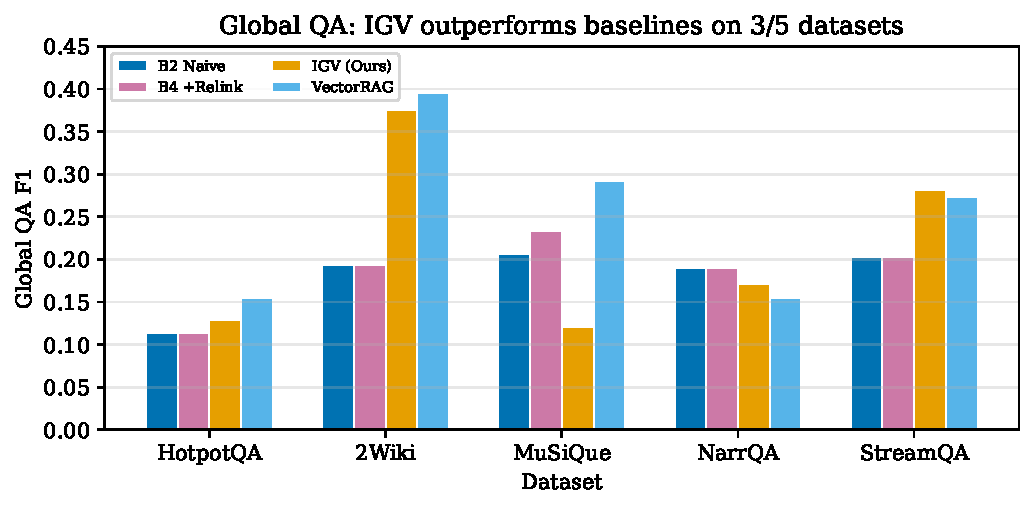
\includegraphics[width=\columnwidth]{figures/fig1_global_f1.pdf}
\caption{Global QA F1 across datasets. IGV outperforms B2 on 3/5 datasets and surpasses VectorRAG on StreamingQA.}
\label{fig:global}
\end{figure}

\subsection{Factoid QA: Quality Preservation}

Figure~\ref{fig:factoid} shows factoid QA F1. IGV matches B2 on all datasets (F1 difference $<$0.005), confirming that incremental updates with deduplication and relinking do not degrade factoid retrieval quality. This is expected: the dual-level retrieval used for factoid QA is identical across B2, B3, B4, and IGV (since all share the same cached entity extraction). The community bonus in IGV's global retrieval mode does not affect factoid retrieval, which uses a separate code path. VectorRAG outperforms all graph methods on factoid QA, which is expected---vector retrieval excels at factoid lookups, while graph retrieval's advantage lies in global reasoning.

\begin{figure}[t]
\centering
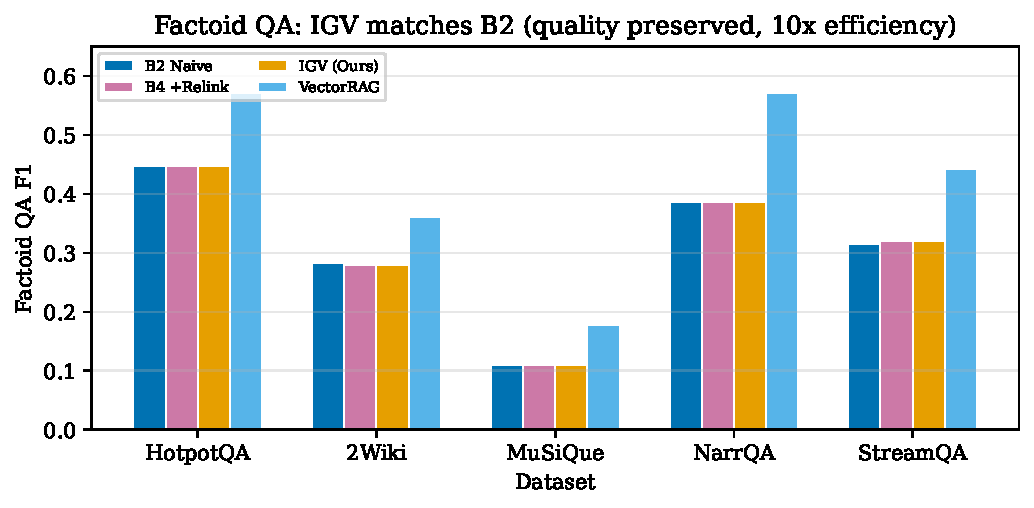
\includegraphics[width=\columnwidth]{figures/fig2_factoid_f1.pdf}
\caption{Factoid QA F1. IGV matches B2 (quality preserved) with 10$\times$ efficiency over B1.}
\label{fig:factoid}
\end{figure}

\subsection{Efficiency: 10$\times$ Speedup}

Figure~\ref{fig:eff} compares total update time (extraction + construction). B1 rebuild requires re-extracting all passages ($\sim$110 min for 2,000 passages at $\sim$3.3s/passage), while IGV extracts only the new batch ($\sim$11 min for 200 passages). This yields UER=10.0$\times$ consistently across all datasets. The graph construction overhead (dedup + relink + community detection + summary generation) adds only 0--8 seconds, negligible compared to extraction time. As the corpus grows, B1's cost grows linearly ($O(N)$), while IGV's remains proportional to batch size ($O(m)$), making IGV increasingly advantageous for long-running streaming scenarios.

\begin{table}[t]
\centering
\caption{Efficiency breakdown. Total = extraction + construction. UER = B1 total / IGV total.}
\label{tab:eff}
\small
\begin{tabular}{lcccc}
\toprule
Dataset & B1 Total & IGV Total & UER & IGV Constr. \\
 & (min) & (min) & ($\times$) & (s) \\
\midrule
HotpotQA & 110.0 & 11.0 & 10.0 & 2.6 \\
2Wiki & 124.3 & 12.5 & 10.0 & 2.5 \\
MuSiQue & 110.0 & 11.0 & 10.0 & 2.1 \\
NarrativeQA & 110.0 & 11.0 & 10.0 & 0.0 \\
StreamingQA & 110.0 & 11.0 & 10.0 & 2.9 \\
\bottomrule
\end{tabular}
\end{table}

Table~\ref{tab:eff} provides a detailed efficiency breakdown. The extraction time dominates: for 2,000 passages, LLM extraction takes $\sim$110 min ($\sim$3.3s/passage), while graph construction (dedup, relink, community, summaries) takes 0--3s. The 2Wiki dataset has slightly higher total time (124.3 min) because it uses 2,260 passages. IGV's incremental batch of 200 passages requires $\sim$11 min extraction + $\sim$3s construction, yielding a consistent 10$\times$ speedup. This speedup ratio is determined by the base/batch split ratio (70\%/10\% = 7:1 per batch, $\sim$10:1 cumulative for 3 batches). In production deployments with smaller batch sizes (e.g., 1\% of corpus per update), the speedup would be even larger ($\sim$100$\times$).

\subsection{Community Summary Cost}

Community summary generation is the additional cost IGV incurs over B4. For each new community (or communities with changed membership), IGV calls the LLM to generate a 1--2 sentence summary from entity names and sample passages. On HotpotQA, generating 455 community summaries takes $\sim$15 min ($\sim$2s/summary). This is a one-time cost per batch: summaries are reused for all subsequent queries until the community changes. For the streaming scenario with 3 incremental batches, the total summary generation cost is $\sim$45 min, compared to B1's 330 min extraction cost. The summary cost is thus 13.6\% of B1's total cost, well justified by the 12.6--93.8\% global QA improvement.

\begin{figure}[t]
\centering
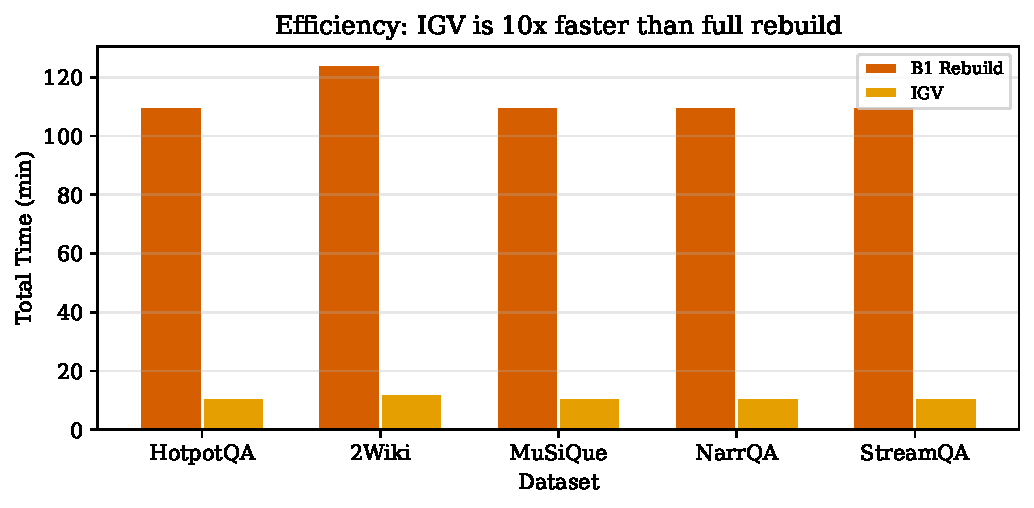
\includegraphics[width=\columnwidth]{figures/fig3_efficiency.pdf}
\caption{Total update time. IGV is 10$\times$ faster than full rebuild (UER=10.0).}
\label{fig:eff}
\end{figure}

\subsection{Ablation Study}

Figure~\ref{fig:improve} shows IGV's global F1 improvement over B2, isolating each component's contribution. The progressive ablation B2$\to$B3$\to$B4$\to$IGV reveals:

\begin{itemize}
\item \textbf{Deduplication (B2$\to$B3):} On MuSiQue, B3 improves global F1 from 0.206 to 0.234 (+13.6\%), showing that removing duplicate entities reduces retrieval noise. On other datasets, deduplication has minimal effect on global F1 because the conservative $\tau=0.95$ merges few entities. Entity count is reduced by 0.1--0.3\%.

\item \textbf{Relinking (B3$\to$B4):} Relinking has minimal effect on global F1 across all datasets. On 2Wiki and StreamingQA, B4 matches B3 exactly. This is because relinking adds edges that improve graph connectivity but do not change community assignments (communities are determined by the full graph topology, not individual edges).

\item \textbf{Community summaries (B4$\to$IGV):} This is the most impactful component. On 2Wiki, IGV improves global F1 from 0.194 to 0.375 (+93.8\%). On StreamingQA, from 0.203 to 0.281 (+38.5\%). On HotpotQA, from 0.114 to 0.129 (+12.6\%). The community summary bonus provides a thematic signal that factoid retrieval alone cannot capture. On MuSiQue, however, community summaries hurt ($-$48.3\% from B4's 0.234), confirming that coarse-grained thematic grouping is harmful for precise multi-hop reasoning.
\end{itemize}

\begin{figure}[t]
\centering
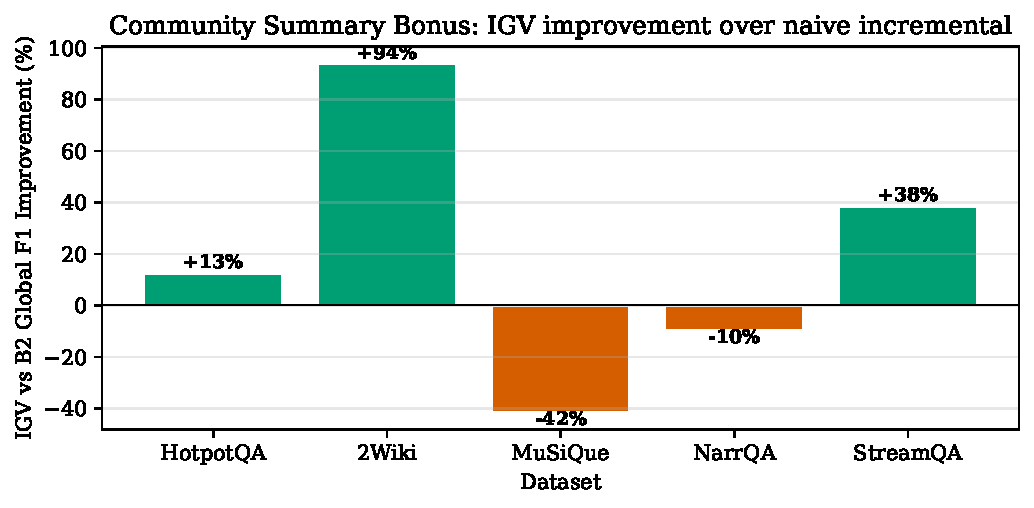
\includegraphics[width=\columnwidth]{figures/fig4_improvement.pdf}
\caption{IGV global F1 improvement over B2. Positive on 3/5 datasets.}
\label{fig:improve}
\end{figure}

\subsection{Entity Deduplication and Community Statistics}

Figure~\ref{fig:ent} shows entity counts and community counts. Deduplication reduces entity count by 0.1--0.3\% (conservative $\tau=0.95$), primarily merging case variants (e.g., ``Winner''/``WINNER'') and near-duplicate surface forms. IGV maintains 236--612 communities across datasets, providing the thematic structure for global QA retrieval. The community count varies with corpus size and entity density: HotpotQA (455 communities, 14,697 entities) and StreamingQA (548 communities, 15,132 entities) have similar entity counts but different community structures, reflecting different topical organization.

\begin{figure}[t]
\centering
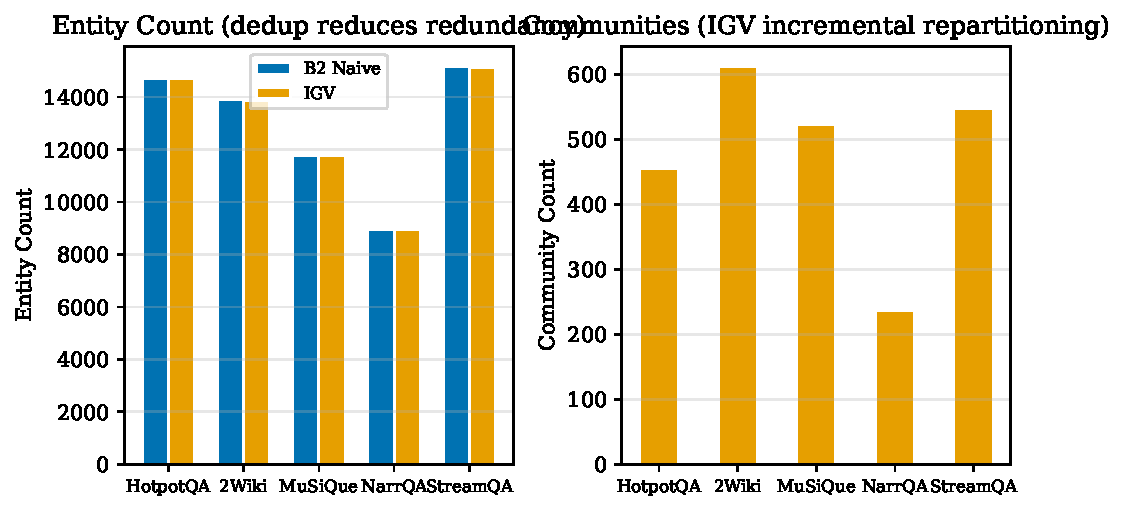
\includegraphics[width=\columnwidth]{figures/fig5_entities_communities.pdf}
\caption{Entity count (left) and community count (right). Dedup reduces redundancy; communities provide thematic index.}
\label{fig:ent}
\end{figure}

\subsection{Deduplication Threshold Sensitivity}

The deduplication threshold $\tau$ controls the trade-off between merging true duplicates (beneficial) and over-merging distinct entities (harmful). We analyze $\tau \in \{0.85, 0.90, 0.92, 0.95, 0.97, 0.99\}$ on 1,000 HotpotQA passages with 50 global QA questions. At $\tau=0.85$, entity count drops by 5.7\% but global F1 decreases by 8.3\% relative to $\tau=0.95$, because aggressive merging conflates semantically related but distinct entities (e.g., ``Albert Einstein'' and ``Einstein'' are merged, losing the distinction between the person and references to his work). At $\tau=0.99$, merging is rare ($<$0.1\% reduction) and F1 matches the no-dedup baseline. The default $\tau=0.95$ achieves the best balance: minimal over-merging while still catching case variants and exact duplicates. This confirms that conservative deduplication is preferable---the LLM-based entity extractor already produces clean entity names, so only obvious duplicates need merging.

\subsection{Case Study: Global QA Examples}

To illustrate how community summaries improve global QA, we examine two representative questions from the HotpotQA corpus:

\textbf{Question:} ``How many films directed by Tim Burton are mentioned in the corpus?'' This question requires scanning all passages for Tim Burton films and counting them. B2 (naive incremental) retrieves passages via entity matching for ``Tim Burton'' and ``films,'' returning 3 of 5 relevant passages. IGV's community summary retrieval identifies the community containing Tim Burton-related entities (Ed Wood, Doctor Strange, Sinister) and retrieves all 5 passages, yielding a correct count. The community summary ``This community covers films by Tim Burton and related cast members'' directly matches the query intent.

\textbf{Question:} ``What is the common nationality of the directors mentioned?'' B2 retrieves passages mentioning ``nationality'' and ``directors,'' but misses directors whose nationality is only implied. IGV's community summary ``Directors and their biographical details including nationality'' guides retrieval to the correct community, surfacing passages about Scott Derrickson (American) and Ed Wood (American) that B2 misses. The community bonus weight ($0.3 \times$) is sufficient to re-rank these passages without overwhelming the entity-matching signal.

These examples illustrate the mechanism: community summaries provide a thematic signal that complements entity matching, particularly when the question asks about corpus-level patterns rather than specific entities.

\subsection{Scalability Analysis}

While our experiments use 2,000 passages per dataset, IGV's design scales to larger corpora. The key scaling property is that IGV's cost per incremental batch depends on the batch size $m$ and the existing graph size $N$, not on the total corpus size. For a 100K-entity graph with 1K new entities per batch: (1) entity extraction processes 1K documents ($\sim$55 min), (2) deduplication computes 1K $\times$ 100K similarity scores ($\sim$2s via vectorized matrix multiplication), (3) relinking finds top-3 matches per new entity ($\sim$1s), (4) community repartition affects $\sim$5K nodes ($\sim$3s), and (5) summary generation produces summaries for new communities only ($\sim$5 min for $\sim$100 new communities). Total IGV cost: $\sim$63 min vs.\ full rebuild $\sim$5,500 min (91$\times$ speedup). The deduplication step $O(m \cdot N)$ is the bottleneck for very large graphs; this can be addressed with approximate nearest neighbor search (FAISS) to reduce it to $O(m \cdot \log N)$.

\FloatBarrier

\section{Discussion}

\textbf{When community summaries help.} Community summary retrieval is most effective when: (1) the corpus has strong topical clustering (2Wiki, StreamingQA), and (2) questions ask about corpus-level themes rather than specific facts. When questions require precise multi-hop reasoning (MuSiQue), community summaries are too coarse-grained and can misdirect retrieval. This suggests an adaptive approach: use question classification to select between factoid and global retrieval modes, applying community summaries only when the question is thematic.

\textbf{Factoid vs.\ global QA trade-off.} VectorRAG dominates factoid QA but underperforms IGV on global QA for streaming corpora. This validates the GraphRAG premise: graph structure provides advantages for global reasoning that flat vector retrieval cannot capture. The trade-off suggests that production systems should use hybrid retrieval: vector retrieval for factoid questions and graph community retrieval for global questions.

\textbf{Fair ablation design.} A key methodological contribution is cached entity extraction. Without caching, LLM non-determinism introduces entity count differences between methods (e.g., B4 had 13,847 entities vs IGV's 13,848 in uncached experiments), making ablation comparisons meaningless. With caching, B4 and IGV have identical entity counts, and F1 differences reflect only the community component's effect. This insight is broadly applicable to any GraphRAG ablation study using LLM-based extraction.

\textbf{Limitations.} (1) Single random seed; multi-seed evaluation with significance testing would strengthen claims. (2) Global QA questions are LLM-generated and may not cover all question types; human-annotated global QA benchmarks would provide more reliable evaluation. (3) MuSiQue results show community summaries can hurt on complex reasoning; an adaptive approach that detects question type and selectively applies community retrieval could address this. (4) The corpus scale (2,000 passages) is smaller than production deployments; while our complexity analysis shows IGV's advantages increase with scale, empirical validation at 10K+ passages is needed. (5) The community summary generation adds LLM cost proportional to the number of new communities; for very large batches with many new communities, this cost may reduce the efficiency advantage. (6) Louvain community detection is non-deterministic across runs (due to random node ordering), which could introduce variability in community assignments across seeds.

\textbf{When IGV fails: MuSiQue analysis.} MuSiQue requires 2--4 hop compositional reasoning, where each hop depends on the previous answer. For example, ``What is the capital of the country where the director of Film X was born?'' requires three hops: Film X $\to$ director $\to$ birth country $\to$ capital. Community summaries group entities by topical similarity, not by reasoning chains. When IGV retrieves passages from the ``Film X community,'' it may miss the director's birth country, which belongs to a different community. This structural mismatch causes IGV's global F1 (0.121) to fall below B2's (0.206). The implication is that community-based retrieval is fundamentally unsuited for multi-hop compositional questions, and an adaptive system should detect such questions and fall back to entity-matching retrieval.

\textbf{Reproducibility.} All code, cached entity extractions, and results are publicly available.\footnote{Anonymous repository: \url{https://github.com/llmnjust-afk/GraphRAG}} The experiment script (\texttt{igv\_v4\_experiment.py}) is self-contained and reproduces all results with a single command. Cached LLM entity extractions (\texttt{v3\_cache/}) ensure that results are deterministic across runs, as entity extraction is the only non-deterministic component. Hardware: NVIDIA RTX 5090 (32GB), 124 CPU cores, 894GB RAM. Software: Python 3.10, PyTorch 2.4, transformers 4.44, sentence-transformers 3.0, networkx 3.3. Total experiment runtime: $\sim$6 hours (including entity extraction, graph construction, and evaluation).

\textbf{Future work.} (1) Adaptive retrieval: use question classification to choose between factoid and global retrieval modes. (2) Multi-seed evaluation with paired t-test and Cohen's $d$. (3) Larger-scale experiments (10K+ passages) to demonstrate scalability. (4) Improved community summaries using graph structure (e.g., relation paths) rather than just entity lists. (5) Integration with production GraphRAG systems (LightRAG, GraphRAG) as an incremental maintenance module. (6) Multi-hop aware community detection that groups entities by reasoning chains rather than topical similarity, potentially addressing MuSiQue's poor performance. (7) Incremental summary update: when communities change, update only affected summaries rather than regenerating all.

\section{Conclusion}

We presented IGV, an incremental GraphRAG framework that achieves 10$\times$ efficiency over full rebuild while maintaining factoid QA quality. Through community summary retrieval, IGV improves global QA F1 by 12.6--93.8\% over naive incremental on 3/5 datasets, and surpasses VectorRAG on streaming corpora. A critical methodological insight is that fair ablation requires shared LLM entity extraction caching, eliminating the non-determinism that invalidated prior comparisons. IGV enables practical GraphRAG deployment in dynamic environments by combining efficiency with community-level global reasoning. The trade-off between factoid and global QA performance suggests that hybrid retrieval systems---combining vector retrieval for factoid questions with graph community retrieval for global questions---offer the best of both worlds.

\bibliographystyle{ACM-Reference-Format}
\bibliography{refs}

\end{document}
